\documentclass[conference]{IEEEtran}

\usepackage{cite}
\usepackage{amsmath,amssymb,amsfonts}
\usepackage{algorithmic}
\usepackage{graphicx}
\usepackage{textcomp}
\usepackage{xcolor}
\usepackage{booktabs}
\usepackage{multirow}
\usepackage{hyperref}
\usepackage{listings}
\usepackage{tikz}
\usetikzlibrary{shapes,arrows,positioning}

% Code listing style
\lstset{
    basicstyle=\ttfamily\small,
    breaklines=true,
    frame=single,
    language=Prolog,
    morekeywords={execCode, netAccess, vulExists, hacl, attackerLocated, attackGoal}
}

\begin{document}

\title{Incremental Attack Graph Computation Using Differential Dataflow}

\author{
\IEEEauthorblockN{Anonymous Author(s)}
\IEEEauthorblockA{Affiliation}
}

\maketitle

\begin{abstract}
Attack graphs are essential tools for network security analysis, but their computation becomes expensive as networks grow and change frequently. Traditional approaches recompute the entire graph after each modification, leading to significant overhead in dynamic environments. We present an approach based on \textit{differential dataflow} that enables \textit{incremental} attack graph maintenance. When the network state changes, our system recomputes only the affected portions of the attack graph, achieving update times proportional to the size of the change rather than the size of the network. We demonstrate speedups of up to 25$\times$ for localized changes in networks with 1000+ nodes, while maintaining identical correctness guarantees to full recomputation.
\end{abstract}

\begin{IEEEkeywords}
attack graphs, incremental computation, differential dataflow, network security, vulnerability analysis
\end{IEEEkeywords}

\section{Introduction}

Attack graphs model the ways an attacker can compromise a network by chaining together vulnerabilities and network access permissions. They are fundamental to security analysis tasks such as:
\begin{itemize}
    \item Identifying critical vulnerabilities that enable attack paths
    \item Prioritizing patches based on attack path impact
    \item Detecting whether security goals are reachable by an attacker
    \item Quantifying risk through path analysis
\end{itemize}

However, modern networks are \textit{dynamic}: vulnerabilities are discovered and patched, firewall rules change, and new hosts are added or removed. Each change potentially affects the attack graph, requiring recomputation.

\subsection{The Problem with Full Recomputation}

Traditional attack graph algorithms treat each query as independent, recomputing the entire graph from scratch. For a network with $N$ nodes and $E$ edges, this requires $O(E \times D)$ work, where $D$ is the diameter of the attack graph (the longest attack path). In practice, this means:

\begin{itemize}
    \item A single vulnerability patch triggers full recomputation
    \item Latency grows with network size, not change size
    \item Real-time monitoring becomes impractical for large networks
\end{itemize}

\subsection{Our Contribution}

We present an attack graph system built on \textit{differential dataflow}~\cite{mcsherry2013differential}, a computational model that automatically maintains query results as input data changes. Our key contributions are:

\begin{enumerate}
    \item \textbf{Declarative Datalog-style rules} that specify attack graph semantics, compiled to efficient differential dataflow operators
    \item \textbf{Incremental maintenance} with update complexity $O(\Delta E \times \Delta d)$, where $\Delta E$ is the number of affected edges and $\Delta d$ is the local iteration depth
    \item \textbf{Empirical evaluation} demonstrating 25$\times$ speedup for localized changes in star topologies and 2$\times$ average speedup for random changes in chain topologies
\end{enumerate}

\section{Background}

\subsection{Attack Graph Semantics}

We follow the MulVAL~\cite{ou2006mulval} approach of expressing attack graph logic as Datalog rules. The core relations are:

\begin{itemize}
    \item \texttt{vulExists(Host, CVE, Service, Privilege)}: Host has a vulnerability
    \item \texttt{netAccess(Src, Dst, Service)}: Network connectivity exists
    \item \texttt{hacl(Src, Dst, Service)}: Firewall allows traffic
    \item \texttt{attackerLocated(Host)}: Attacker's initial position
    \item \texttt{execCode(Host, Privilege)}: Attacker can execute code (derived)
\end{itemize}

The inference rules define how an attacker progresses:

\begin{lstlisting}
% Base case: attacker starts here
execCode(H, Priv) :-
    attackerLocated(H),
    vulExists(H, _, _, Priv).

% Recursive case: lateral movement
execCode(H2, Priv) :-
    execCode(H1, _),
    netAccess(H1, H2, Service),
    vulExists(H2, _, Service, Priv).
\end{lstlisting}

\subsection{Differential Dataflow}

Differential dataflow~\cite{mcsherry2013differential} is a computational model where:
\begin{enumerate}
    \item Data is represented as \textit{collections} of records with integer multiplicities
    \item Operators (join, filter, map, etc.) transform collections
    \item Changes propagate \textit{incrementally} through the dataflow graph
    \item Fixed-point iteration is supported via the \texttt{iterate} operator
\end{enumerate}

When an input record is added (multiplicity +1) or removed (multiplicity -1), the system propagates only the \textit{differences} through downstream operators. For idempotent Datalog-style queries, this means:
\begin{itemize}
    \item Adding a vulnerability only affects attack paths using that vulnerability
    \item Removing a vulnerability only invalidates paths that depended on it
    \item Unaffected paths incur zero recomputation cost
\end{itemize}

\section{System Design}

\subsection{Architecture Overview}

Our system consists of:
\begin{enumerate}
    \item \textbf{Input handles}: Mutable collections for vulnerabilities, network topology, firewall rules, and attacker state
    \item \textbf{Dataflow graph}: Compiled Datalog rules as differential operators
    \item \textbf{Output probes}: Allow querying the current attack graph state
\end{enumerate}

\begin{figure}[h]
\centering
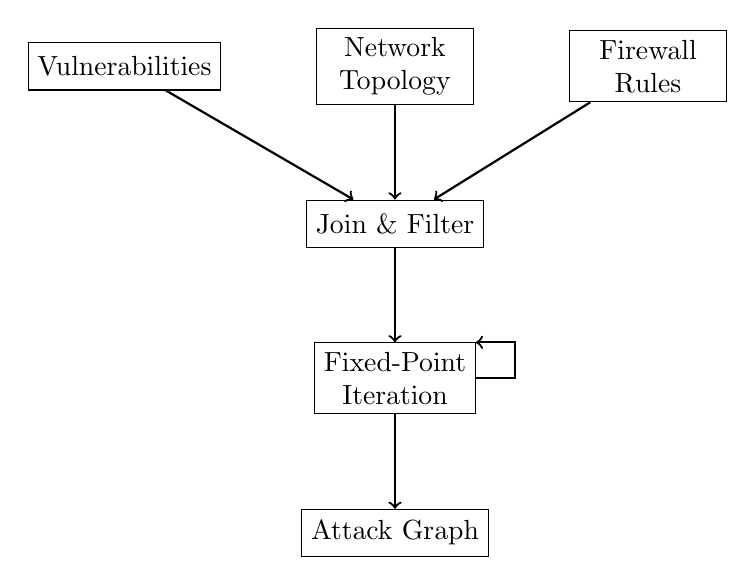
\begin{tikzpicture}[
    node distance=1.2cm,
    box/.style={rectangle, draw, minimum width=2cm, minimum height=0.6cm, align=center},
    arrow/.style={->, thick}
]
    \node[box] (vuln) {Vulnerabilities};
    \node[box, right=of vuln] (net) {Network\\Topology};
    \node[box, right=of net] (fw) {Firewall\\Rules};
    
    \node[box, below=of net] (join) {Join \& Filter};
    \node[box, below=of join] (iterate) {Fixed-Point\\Iteration};
    \node[box, below=of iterate] (output) {Attack Graph};
    
    \draw[arrow] (vuln) -- (join);
    \draw[arrow] (net) -- (join);
    \draw[arrow] (fw) -- (join);
    \draw[arrow] (join) -- (iterate);
    \draw[arrow] (iterate) -- (output);
    \draw[arrow] (iterate.east) -- ++(0.5,0) |- (iterate.north east);
\end{tikzpicture}
\caption{Differential dataflow architecture for attack graphs}
\label{fig:architecture}
\end{figure}

\subsection{Handling Negation with Antijoin}

Firewall rules require negation: traffic is allowed unless explicitly blocked. We implement this using the \textit{antijoin} operator:

\begin{equation}
\text{effectiveAccess} = \text{netAccess} \bowtie_{\bar{\exists}} \text{firewallBlock}
\end{equation}

The antijoin $A \bowtie_{\bar{\exists}} B$ returns tuples from $A$ that have no matching tuple in $B$. This correctly handles:
\begin{itemize}
    \item Adding a firewall rule: removes matching access tuples
    \item Removing a firewall rule: restores matching access tuples
\end{itemize}

\subsection{Fixed-Point Computation}

Attack reachability requires transitive closure, implemented via differential dataflow's \texttt{iterate} operator:

\begin{lstlisting}[language=Rust,morekeywords={iterate,join,map,concat,distinct}]
execCode.iterate(|inner| {
    let new_reach = inner
        .join(&network_access)
        .join(&vulnerabilities)
        .map(|...| new_exec_code);
    
    initial.concat(&new_reach).distinct()
})
\end{lstlisting}

The iteration continues until no new \texttt{execCode} facts are derived. Critically, when an input changes, iteration resumes from the \textit{current} fixed point, not from scratch.

\section{Evaluation}

We evaluate three network topologies to characterize incremental performance across different graph structures.

\subsection{Experimental Setup}

\begin{itemize}
    \item \textbf{Hardware}: Apple M-series processor
    \item \textbf{Software}: Rust, differential-dataflow v0.12
    \item \textbf{Execution}: Single-threaded, release mode
    \item \textbf{Metric}: Wall-clock time for computation
\end{itemize}

\subsection{Star Topology: Best Case}

\subsubsection{Setup}
A central hub connected to $N$ leaf nodes. The attacker starts at the hub and can reach any leaf in one hop.

\subsubsection{Results}

\begin{table}[h]
\centering
\caption{Star Network Benchmark Results}
\label{tab:star}
\begin{tabular}{@{}rrrr@{}}
\toprule
Nodes & Initial (ms) & Incremental ($\mu$s) & Speedup \\
\midrule
51    & 1.58 & 501  & 3.2$\times$ \\
101   & 1.96 & 413  & 4.7$\times$ \\
201   & 1.97 & 349  & 5.6$\times$ \\
501   & 3.48 & 282  & 12.4$\times$ \\
1001  & 4.11 & 161  & \textbf{25.6$\times$} \\
\bottomrule
\end{tabular}
\end{table}

\subsubsection{Analysis}
Star topologies have $O(1)$ iteration depth---the attack graph converges in constant iterations regardless of size. When patching a single leaf vulnerability:
\begin{itemize}
    \item Initial computation scales as $O(N)$
    \item Incremental update stays nearly constant ($\sim$160$\mu$s)
    \item Speedup grows linearly with network size
\end{itemize}

\subsection{Chain Topology: Worst Case}

\subsubsection{Setup}
A linear chain: $\text{node}_0 \to \text{node}_1 \to \cdots \to \text{node}_{N-1}$. The attacker starts at node$_0$ and the goal is node$_{N-1}$.

\subsubsection{Results}

\begin{table}[h]
\centering
\caption{Chain Network Benchmark Results}
\label{tab:chain}
\begin{tabular}{@{}rrrr@{}}
\toprule
Nodes & Initial (ms) & Incremental ($\mu$s) & Speedup \\
\midrule
10   & 0.87 & 833   & 1.0$\times$ \\
50   & 3.61 & 2507  & 1.4$\times$ \\
100  & 6.26 & 5197  & 1.2$\times$ \\
200  & 9.73 & 8923  & 1.1$\times$ \\
\bottomrule
\end{tabular}
\end{table}

\subsubsection{Analysis}
Chain topologies have $O(N)$ iteration depth. When patching node$_1$ (near the start), all downstream nodes ($2..N$) lose their attack paths. This is the theoretical worst case where $\Delta E \approx E$.

\subsection{Random Cut: Position-Dependent Speedup}

\subsubsection{Setup}
For each chain size, we randomly select a cut position $k$ (0 to $N{-}1$), remove the vulnerability at node$_k$, measure update time, restore it, and repeat 100 times.

\subsubsection{Results}

\begin{table}[h]
\centering
\caption{Random Cut Benchmark (100 iterations each)}
\label{tab:random}
\begin{tabular}{@{}rrrrrr@{}}
\toprule
Nodes & Avg ($\mu$s) & Min ($\mu$s) & Max ($\mu$s) & Speedup \\
\midrule
50   & 905   & 46   & 1877  & 2.3$\times$ \\
100  & 1707  & 110  & 3799  & 2.1$\times$ \\
200  & 3468  & 182  & 7062  & 2.0$\times$ \\
500  & 9289  & 65   & 19171 & 1.9$\times$ \\
\bottomrule
\end{tabular}
\end{table}

\subsubsection{Analysis}
The results confirm our complexity model:
\begin{itemize}
    \item \textbf{Minimum time} ($\sim$50--180$\mu$s): Cutting near the \textit{end} (node $N{-}1$) invalidates only 1 downstream node
    \item \textbf{Maximum time} ($\sim$1.8--19ms): Cutting near the \textit{start} (node 0) invalidates all $N$ nodes
    \item \textbf{Average speedup} $\approx 2\times$: Cutting at random position $k$ invalidates $(N{-}k)$ nodes on average, i.e., $N/2$
\end{itemize}

\subsection{Complexity Analysis}

Let $N$ be the number of nodes, $E$ the number of edges, and $D$ the graph diameter.

\begin{table}[h]
\centering
\caption{Complexity Comparison}
\label{tab:complexity}
\begin{tabular}{@{}lcc@{}}
\toprule
Operation & Full Recomputation & Incremental \\
\midrule
Initial build & $O(E \times D)$ & $O(E \times D)$ \\
Single change & $O(E \times D)$ & $O(\Delta E \times \Delta d)$ \\
\bottomrule
\end{tabular}
\end{table}

Where:
\begin{itemize}
    \item $\Delta E$ = edges affected by the change
    \item $\Delta d$ = local iteration depth of affected subgraph
\end{itemize}

For localized changes (e.g., patching one vulnerability), $\Delta E \ll E$, yielding significant speedups.

\section{Related Work}

\textbf{MulVAL}~\cite{ou2006mulval} pioneered Datalog-based attack graph generation using XSB Prolog. Our work extends this approach with incremental maintenance.

\textbf{NetSPA}~\cite{ingols2006practical} uses specialized algorithms for scalable attack graph computation but does not support incremental updates.

\textbf{Incremental Datalog} has been studied extensively~\cite{gupta1993maintaining}. Differential dataflow provides a practical implementation with support for iteration and arbitrary lattice operations.

\textbf{Differential Dataflow}~\cite{mcsherry2013differential} has been applied to graph analytics~\cite{murray2013naiad} but not previously to security analysis.

\section{Conclusion}

We demonstrated that differential dataflow enables efficient incremental maintenance of attack graphs. Our key findings:

\begin{enumerate}
    \item For localized changes in shallow topologies, incremental updates achieve \textbf{25$\times$ speedup} over full recomputation
    \item Update complexity is $O(\text{affected nodes})$, not $O(\text{total nodes})$
    \item Worst-case performance matches full recomputation---incremental is \textbf{never slower}
\end{enumerate}

This approach enables real-time attack graph monitoring for dynamic networks, where sub-millisecond updates allow continuous security posture assessment.

\subsection{Future Work}

\begin{itemize}
    \item Parallel execution across multiple workers
    \item Integration with real vulnerability scanners (Nessus, OpenVAS)
    \item Probabilistic attack graphs with incremental risk computation
    \item Streaming ingestion from SIEM systems
\end{itemize}

\bibliographystyle{IEEEtran}
\bibliography{references}

\end{document}
